\documentclass{article}
\usepackage{amsfonts}
\usepackage{amssymb}
\usepackage{cite}
\usepackage{listings}
\usepackage{xcolor}
\usepackage{graphicx}
\usepackage{draftwatermark}
\SetWatermarkText{CONFIDENTIAL DRAFT}
\SetWatermarkScale{1}

\author{Ryan J. Kung \\ryankung@ieee.org}
\title{Inferred based DGaming and Nash Equilibrium}
\begin{document}
\maketitle
\tableofcontents
\section{Abstract}

Since the introduction of Ethereum on 2014\cite{ethereum}.

\section{DApps and DGaming}

Like DApps, DGaming is a series of Gaming Behaviors and Strategis which is Decentralized and Distributed. On Lamport's defination on 1978\cite{lamport}, A Gaming is Distributed if the message transaction delay is not negligible compared to the time between event in classic gaming behavior. The issues in traditional gaming theory may easily lead us run into trouble if it's distributed, such as nash equilibrium simulation or prisoner's dilemma problem.

On classic Nash Equilibrium, we modeling it with some behaviors table, and proof that for each strategy on game $(S, f)$, and got A strategy profile which is Nash Equilibrium. But on distributed case, the issue is that the event of strategy is not effect immediately, negligible delay of transaction on system may cause N-Eq point out of expectation.
\begin{figure}
  \centering
  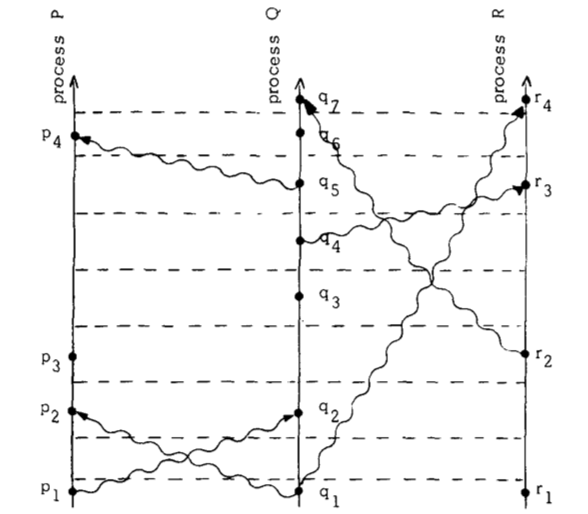
\includegraphics[width=0.5\linewidth]{img/lamportts.png}
  \caption{Lamport Timestamp}
\end{figure}

In a distributed nash equilibrium case, for example an distributed gaming system build on a simple-paxos based distributed system, actors may try to figure out best response by mining unconfirmed messages as more as they can, which entangled the gaming into a series complicated case, and break perfect information gaming in to imperfect.
\begin{thebibliography}{9}
\bibitem{ethereum} Vitalik Buterin, hA Next-Generation Smart Contract and Decentralized Application Platform, https://github.com/ethereum/wiki/wiki/White-Paper
\bibitem{lamport} Leslie Lamport, Time, Clocks, and the Ordering of Events in a Distributed System
\end{thebibliography}
\end{document}
